\documentclass[frenchb]{article}
\usepackage[T1]{fontenc}
%Pour utilisation sous unix
\usepackage[utf8]{inputenc}
%\usepackage[utf8x]{inputenc}
\usepackage{a4wide}
\usepackage{graphicx}
\usepackage{amssymb}
\usepackage{color}
%\usepackage[latin1]{inputenc}
\usepackage{babel}
\usepackage{caption}
\usepackage{subcaption}

\begin{document}
	
	\begin{figure}[t]
		\centering
		%\includegraphics[width=7cm]{n7.png}
	\end{figure}
	
	\title{\vspace{4cm} \textbf{Rapport projet Calcul Scientifique et Analyse de Données Partie 3}}
	\author{ALOUANE Issam\\ BOUAM Adam\\ DABROWSKI Rémi\\ }
	\date{\vspace{9cm} Département Sciences du Numérique - Première année \\
		2021-2022 }
	
	\maketitle
	
	\newpage
	\tableofcontents
	\listoffigures
	
	\newpage
	\section{Introduction}{
	La troisième et dernière partie de ce projet a pour but de reconstruire les visages grâce à deux classifieurs : les k-plus-proches voisins et la méthode bayésienne. Dans un premier temps nous les utiliserons pour la reconnaissance des visages. Puis nous étudierons la reconstruction des visages et pour finir, nous évaluerons la performance de chacun.
	
	}
	
	\section{Reconnaissance sans masque}{
		
		
	}
	\subsection{Réalisation}
	Après avoir adapté les algorithmes de calcul du k-plus-proche voisin et de la méthode bayésienne, 
	Nous obtenons les figures suivantes :
	
		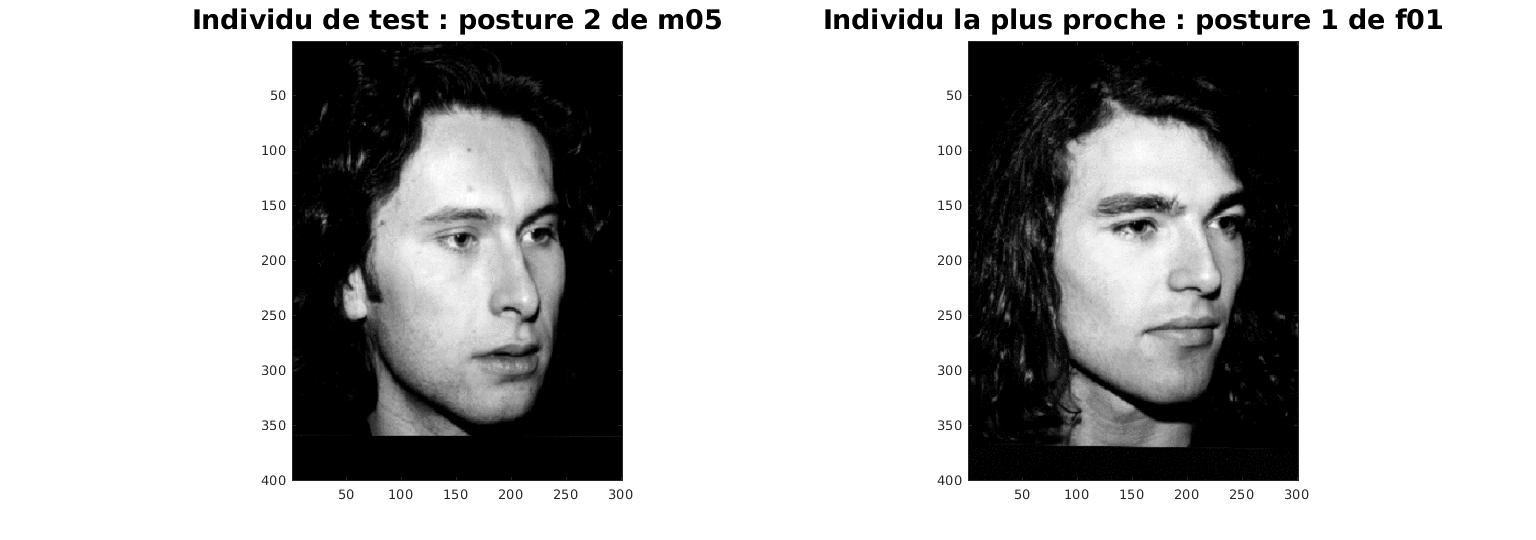
\includegraphics[scale=.2]{1.jpg}
		
		
	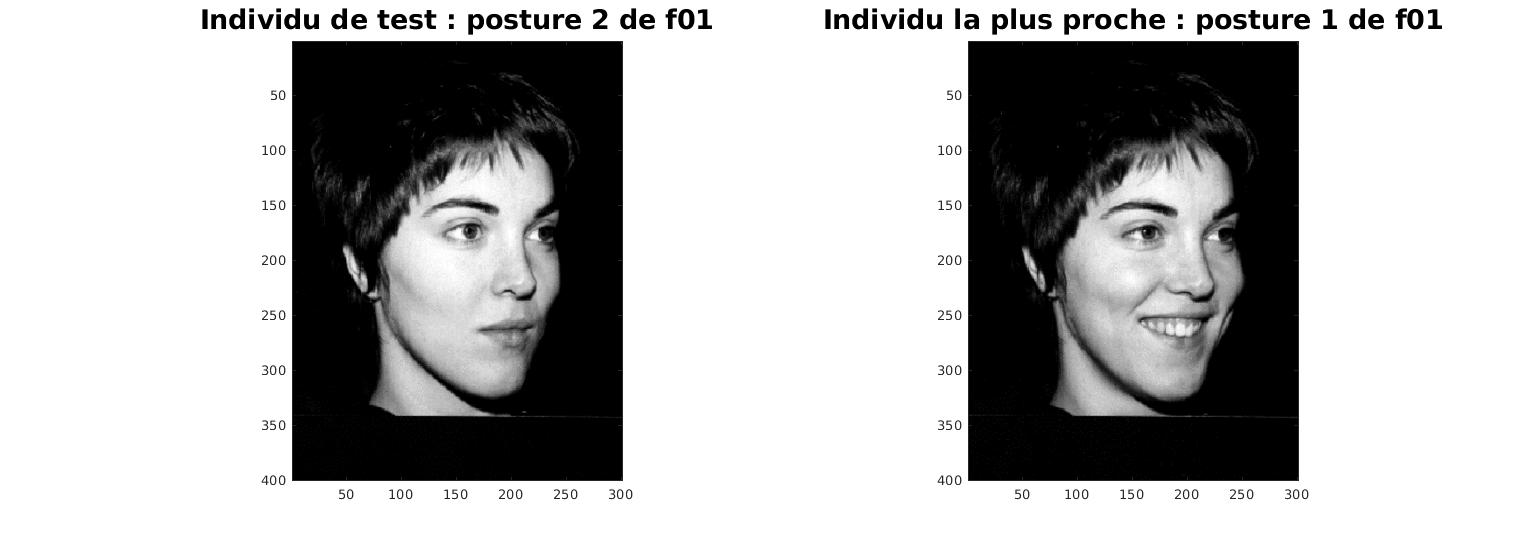
\includegraphics[scale=.2]{2.jpg}
	

	\subsection{Question 3.3}
	La méthode des k-plus-proches voisins dépend de k, ici nous avons déterminé k = 1.
	De plus, les classifieurs de notre étude dépendent des données de la base de référence. Ainsi, ils dépendent du nombre de composantes spectrales choisies. Afin d'avoir des résultats convaincants nous avons choisi ce nombre en fonction d'un haut contraste voulu.

	\newpage
	
	\section{Reconnaissance avec masque}
	\subsection{Exemples obtenus}
	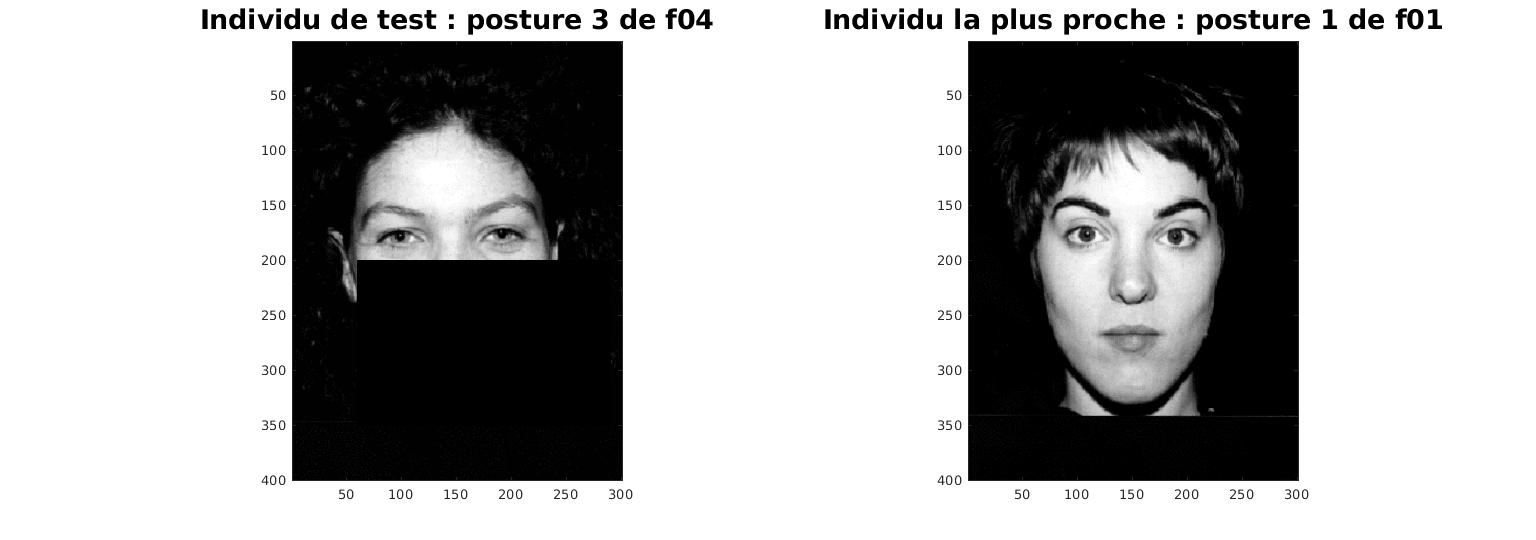
\includegraphics[scale=.2]{3.jpg}
		
	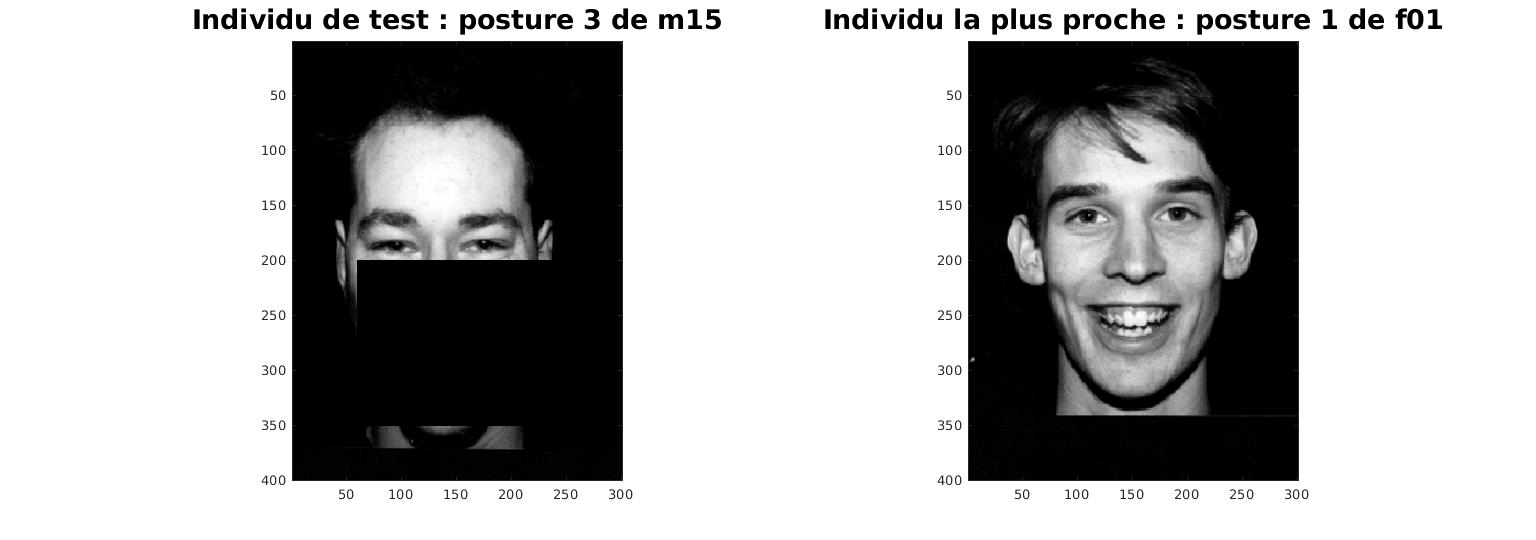
\includegraphics[scale=.2]{4.jpg}
	
	
	
	
	\section{Reconstruction des visages}
	\subsection{Réalisation}
	Voici certains des tests que nous avons effectué :
	
	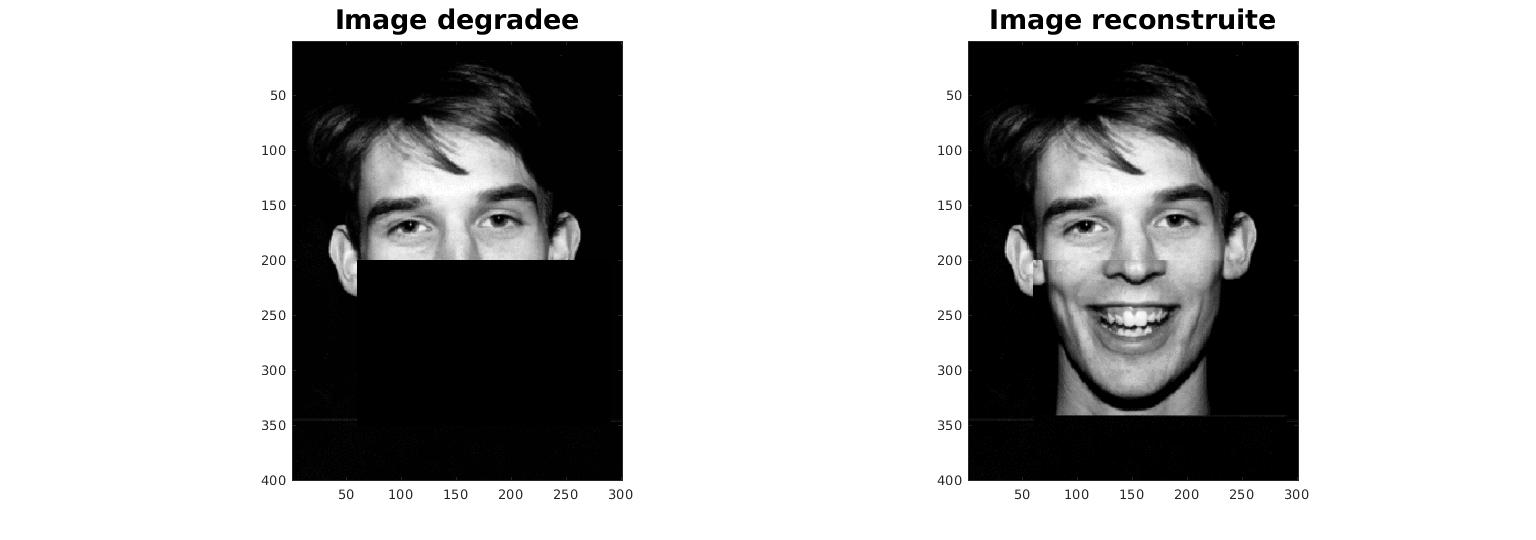
\includegraphics[scale=.2]{5.jpg}
		
	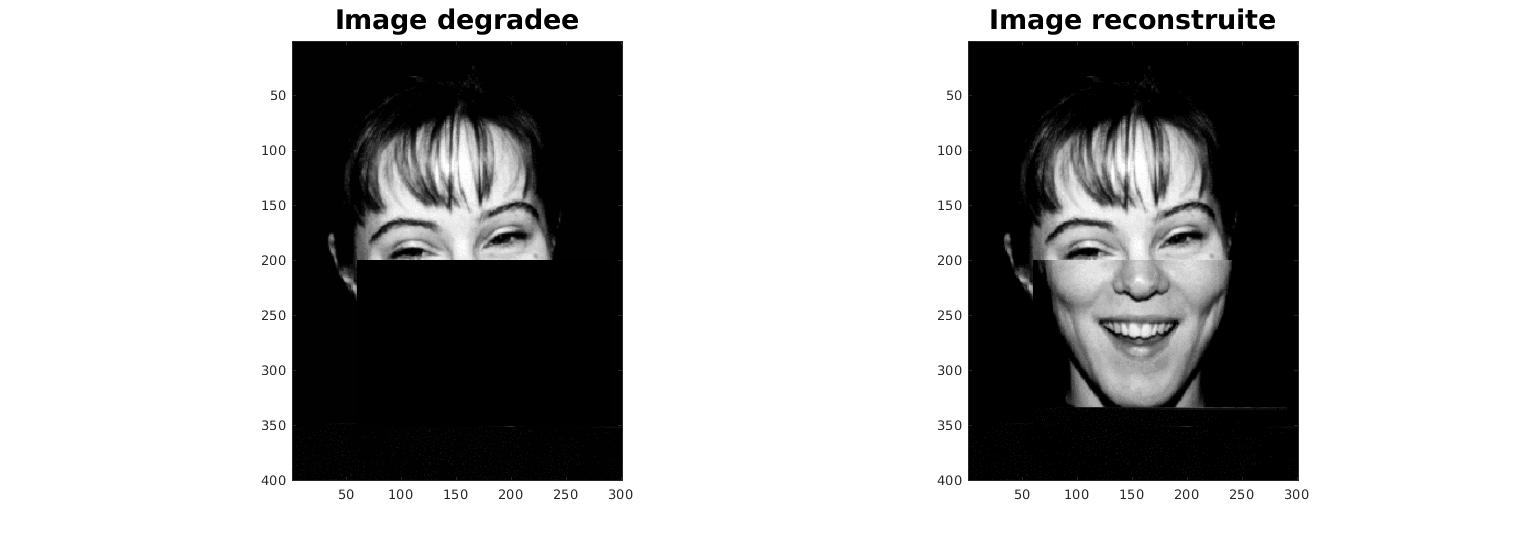
\includegraphics[scale=.2]{6.jpg}
	\newpage
	\section{Evaluation des classifieurs}
	Pour notre étude nous avons tout d'abord choisi de travailler avec 16 personnes dans notre base de données et 4 postures.
	Avec la méthode de plus proche voisin :
	Lorsque le visage est dans la base de donnée le classifieur détermine bien la bonne personne mais peut lui assigner une posture différente. S'il n'y est pas par contre, le résultat n'est pas concluant. Par exemple:
	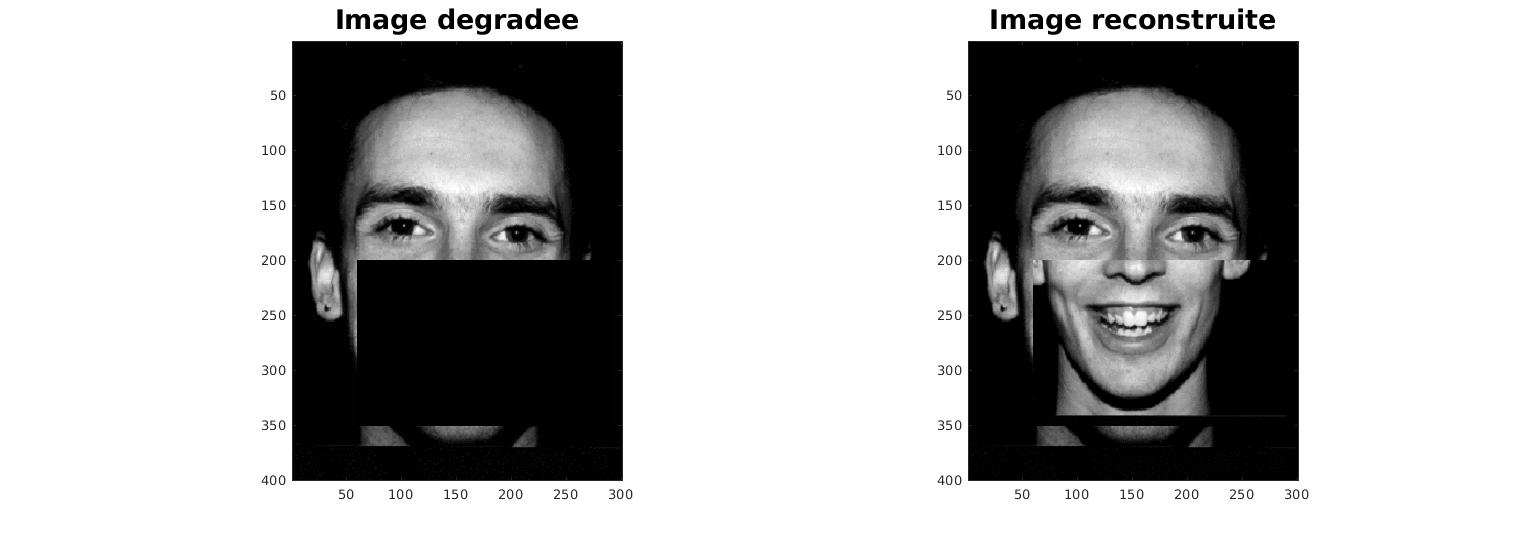
\includegraphics[scale=.2]{nul.jpg}
	
	
	Par la suite nous avons testé avec 24 visages et toutes les postures.
	Dans ce cas, la méthode kppv s'avère encore plus efficace en donnant un visage cohérent à (presque) chaque tentative ce qui correspond avec nos attentes.
	
	- 
	
	
\end{document}